% !TeX spellcheck = ru_RU
% !TEX root = vkr.tex

\section{Обзор}

Данный раздел содержит обзор сущностей, взаимодействующих с глобальной очередью, инструментов бенчмаркинга.

\subsection{Многопоточный рантайм tokio}

При инстанциации рантайм создает определенное количество системных потоков для так называемого блокирующего пулла, призванного исполнять ресурсоемкие задачи. Всего создается \verb|worker_threads| + \verb|max_blocking_threads| потоков, где

\begin{itemize}
    \item \verb|worker_threads| --- количество потоков предназначенных для исполнения асинхронных задач
    \item \verb|max_blocking_threads| --- максимальное количество блокирующих потоков
\end{itemize}

\begin{figure}[H]
    \begin{center}
        \makebox[\textwidth]{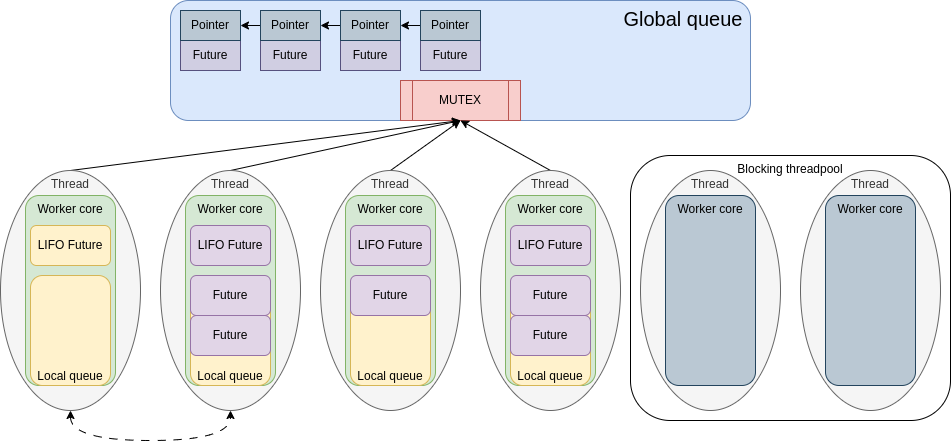
\includegraphics[scale=0.55]{pictures/tokio.arch.png}}
    \end{center}

    \caption{Упрощенное представление многопоточного рантайма}
    \label{fig:tokio:arch}
\end{figure}

Блокирующие потоки ожидают определенный период, 10 секунд если не специфицировано иначе, поступления задач после чего прекращают свое исполнение.

\verb|Воркер|, так называется сущность ассоциированная с каждым из оставшихся \verb|worker_threads| потоков с помощью размещения в локальной для этих поток переменной так называемого \verb|ядра воркера| --- структуры, необходимой для исполнения асинхронных задач, включающей \verb|локальную очередь|, хендлер \verb|глобальной очереди| и тому подобное.

\verb|Локальная очередь| воркера выступает в качестве кэша его задач, имеет фиксированный размер и предполагает добавление задач исключительно из потока владельца. Однако, изъятие из нее может быть осуществлено потоками других воркеров при нехватке оным собственных задач --- процесс называемый стилингом. Все это: фиксированный размер и производитель в единственном количестве позволяет ей иметь lock free алгоритм взаимодействия. В случае переполнения часть задач перемещается воркером в глобальную очередь.

\verb|Глобальная очередь| или \verb|inject queue| представляет собой коллекцию задач ожидающих исполнения. Наполняется она при спавнинге задачи вне контекста воркера или при переполнении локальной очереди воркеров. Реализована с помощью интрузивного связного списка, защищенного мьютексом.

Исполнить асинхронное замыкание пользователь может несколькими способами:

\begin{itemize}
    \item \verb|block_on| --- метод инстанса рантайма позволяющий заблокировать поток приложения на исполнении определенного асинхронной задачи
    \item \verb|tokio::spawn| --- функция позволяющая поместить асинхронное замыкание в одну из очередей рантайма. Вызов ее должен быть совершен в его контексте --- в одном из потоков, управляемых рантаймом, в методе \verb|block_on| или промежутке жизни объекта \verb|EnterGuard|. От места вызова будет зависеть, в какую очередь будет помещена задача: в случае потока воркер --- в локальную очередь, иначе --- глобальную
\end{itemize}

\subsubsection{Выбор задачи}

Логика поиска воркером задачи для исполнения отражена на листинге \ref{listing:next_task}.

\begin{listing}[H]
    \begin{minted}{rust}
fn next_task(&mut self) -> Option<Notified> {
    if self.tick % self.global_queue_interval == 0 {
        return next_remote_task()
                .or_else(|| self.next_local_task())
    }
    if Some(task) = self.next_local_task()  {
        return Some(task);
    }
    if inject().is_empty() {
        return None;
    }
    let (head, tail) = inject().pop_n(self.can_take());
    self.run_queue.push_back(tail);
    return head
}
    \end{minted}

    \caption{Логика выбора задачи}
    \label{listing:next_task}
\end{listing}

И осуществляется в следующем порядке: раз в определенное, конфигурируемое рантаймом, число тиков --- мера времени воркера, он пытается взять задачу из глобальной очереди, иначе --- из локальной, в остальное время проверке подлежит локальная, после --- глобальная очереди.

\subsection{Цикл работы воркера}

Алгоритм рабочего цикла воркера отражен на листинге \ref{listing:worker:run}.

\begin{listing}[H]
    \begin{minted}{rust}
fn run() {
    while !is_shutdown() {
        core.tick();
        if let Some(task) = core.next_task() {
            self.run_task(task, core);
            continue;
        }
        if let Some(task) = core.steal_work() {
            self.run_task(task, core);
            continue;
        }
        self.park(core)
    }
}
    \end{minted}

    \caption{Логика выбора следующей задачи}
    \label{listing:worker:run}
\end{listing}

А именно, воркер отсчитывает тик, затем пытается найти задачу, после чего пытается украсть задачи у других воркеров. В случае неудачи он паркует поток.

\subsection{Бенчмаркинг}

Для измерений производительности была использована библиотека \verb|criterion|\footnote{\href{https://github.com/bheisler/criterion.rs}{Репозиторий} проекта criterion (Дата обращения: 4.1.2025)}. Так как она популярна, имеет обширную документацию и используется в \verb|tokio|.

\subsection{Изменения шедулера языка Go}

Как было отмечено ранее, алгоритмы шедулинга в \verb|tokio| были созданы с оглядкой на реализацию рантайма языка \verb|Go|. С тех пор, никаких изменений с точки зрения структуры распределения задач рантайм Go не претерпел Таким образом, все рантаймы предполагают наличие локальных очередей у воркеров и одной глобальной очереди.
